\section{Backend REST API and Application Server Architecture}
\label{sec:backend_server}

\subsection{What the Backend Does}
The backend is the middle layer between the dashboard (front end) and the files and scripts that collect system information. The dashboard asks the backend for information or asks it to perform an action. The backend checks the request, reads or updates the appropriate files, runs a script when needed, and sends a response (usually JSON) back to the dashboard.

The Flask application listens locally on \texttt{127.0.0.1}. Its routes are grouped by purpose: status and system information, metrics, alerts, collector controls, pipeline execution, and configuration.

\subsection{Threads, Locks, and the Startup Settings}
\textbf{Threading -- problem and solution:} A scheduled data-processing job should not stop the web application from responding to dashboard requests while it waits to run. The code solves this by placing the periodic pipeline task in a separate background thread. The thread reads the configured interval, waits, and then starts the pipeline. It is a \texttt{daemon} thread, so it does not keep the application alive after the main program exits.

\textbf{Thread lock -- problem and solution:} A user might press the Run Pipeline button repeatedly, or a manual request might arrive just as the automatic timer starts a run. Without protection, two pipeline executions could overlap, duplicate work, compete for CPU and interfere with files being processed. The \texttt{pipeline\_lock} acts like a one-at-a-time gate: both the timer and \texttt{POST /api/pipeline/run} must acquire it before starting. If the lock is already held, the new request is rejected (or the timer skips that run). This guarantees that only one pipeline execution is active at a time; it does not permanently block later runs. The lock is released even if execution fails.

\textbf{Numerical-library thread limits -- problem and solution:} Pandas and NumPy can use numerical libraries that create their own worker threads. Too many extra threads can compete for CPU time and add overhead. Before importing these libraries, the code sets \texttt{OPENBLAS\_NUM\_THREADS}, \texttt{OMP\_NUM\_THREADS}, and \texttt{MKL\_NUM\_THREADS} to \texttt{1} when not already set. This limits those library thread pools and helps keep resource use predictable.

\subsection{Important File and Data Operations}
\textbf{\texttt{get\_file\_path} -- problem and solution:} Several endpoints need to locate files in the data folders. Rebuilding those paths separately in many places makes the code repetitive and increases the chance of looking in the wrong folder. This helper provides one consistent way to find a file in \texttt{data/} and its subfolders. During testing, fixture files can be used only when \texttt{SYSMON\_USE\_FIXTURES=1} is enabled; normal operation therefore continues to use real data.

\textbf{Atomic writes -- problem and solution:} If a program writes directly over an existing JSON or configuration file, the file is usually emptied first and then filled. A reader that tries to open it during that brief write could see incomplete content; for JSON, parsing that partial content may fail. The functions \texttt{atomic\_write\_json} and \texttt{atomic\_write\_config} avoid this by writing the complete new content to a temporary file in the same directory, then replacing the old file with \texttt{os.replace}. A reader therefore sees the previous complete version or the new complete version, rather than a half-written file. Temporary files are cleaned up if the write fails. The JSON function is used for acknowledgement data, while the configuration function is used for INI files. \textit{This protects file integrity; it does not by itself coordinate two writers changing the same data at once. A separate lock would be needed to prevent one simultaneous update from overwriting another.}

\textbf{Why Pandas instead of manually processing the CSV with \texttt{open()} -- problem and solution:} The metrics endpoint converts columns to numbers, finds a time range, sorts samples, combines fresh raw readings, groups readings into buckets, and calculates averages. A basic \texttt{open()} loop would typically scan rows and implement these steps manually, using extra loops and intermediate data structures. Finding recent records may still require reading earlier rows. Pandas treats the CSV as a table and provides optimised operations for filtering, sorting, and resampling, making this combined workload simpler and generally more efficient. This does not mean \texttt{open()} is always slow; Pandas is simply better suited to these data-analysis operations. In this implementation, \texttt{read\_csv()} still loads the clean CSV into memory before filtering. The code continues to use \texttt{open()} for simple JSON and PID files and the \texttt{csv} module for alerts.

\subsection{Metrics Optimisation and Bucket Sizes}
The metrics endpoint supports three time ranges. The code keeps a shorter sampling step for a short view and reduces the number of returned points for longer views:

\begin{center}
\small
\begin{tabularx}{0.78\linewidth}{@{}lrrl@{}}
\toprule
\textbf{Requested range} & \textbf{Window} & \textbf{Step} & \textbf{Bucket size}\\
\midrule
\texttt{1h} & 1 hour & 5 seconds & No resampling\\
\texttt{24h} & 24 hours & 60 seconds & 1 minute\\
\texttt{7d} & 7 days & 600 seconds & 10 minutes\\
\bottomrule
\end{tabularx}
\end{center}

\textbf{Downsampling -- problem and solution:} Sending every recorded point for a long time range can create a very large response. The browser then has to receive, store, and draw all those points. This can increase transfer time and memory use, slow down charts, and make the dashboard appear frozen when the history is large. The backend addresses this with \textbf{downsampling}: it groups readings into fixed time buckets and returns one representative point for each bucket instead of every original point. For the 24-hour view, readings in each one-minute bucket become one result; for the seven-day view, readings in each ten-minute bucket become one result. Numeric measurements are averaged, quality flags such as \texttt{is\_gap} and \texttt{is\_outlier} use the maximum value so that a flagged reading is not hidden, and the timestamp text keeps the last value in the bucket. The shorter one-hour live view is not resampled and retains its five-second step, so recent changes remain visible. This reduces the amount of data sent to and drawn by the browser while preserving the overall trend. For the live view, the endpoint also appends new raw samples that have not yet reached the cleaned file, avoiding a wait for the next cleaning run.

\textbf{Important distinction:} in the current implementation, Pandas first loads the clean metrics CSV and then applies the requested time filter and downsampling. Therefore, downsampling directly reduces the data returned to the browser and the work required to display it; it does not by itself prevent a very large source CSV from using memory while being loaded by the backend. A further improvement for much larger datasets would be to read only the recent portion of the file, process it in chunks, or maintain pre-aggregated data for longer time ranges.

\subsection{Status, Alerts, Acknowledgement, and Configuration}
\textbf{Get status -- \texttt{GET /api/status}:} Reports the server time, whether the collector appears to be running, its process ID when available, the newest sample time found in the data, and the last recorded pipeline result. It checks the status shell script and reads the relevant status/data files.

\textbf{Get system and stats:} \texttt{GET /api/system} returns saved machine details such as CPU core information; \texttt{GET /api/stats} returns the saved statistics JSON. If a file is missing or cannot be read, these endpoints return an empty JSON object rather than stopping the whole server.

\textbf{Acknowledgement -- problem and solution:} Without saving acknowledgement state, alerts that a user has already reviewed could appear unacknowledged again after a refresh. \texttt{GET /api/alerts} therefore reads the alert rows and the saved list of acknowledged IDs, then marks each alert accordingly. When the user acknowledges selected alerts or all alerts, the dashboard sends \texttt{POST /api/alerts/ack}. The backend validates the IDs, updates the saved set, and uses the atomic JSON writer so the acknowledgement file is not exposed in a half-written state. Acknowledgement records that an alert has been seen; it does not delete the alert itself.

\textbf{Pipeline:} The pipeline is the processing script launched by \texttt{run\_pipeline.sh}. It is run periodically by the background timer and can also be requested manually. The lock prevents the timer and a manual request from starting overlapping runs. The backend waits for the script to finish (up to the configured timeout), then returns success or an error response. The status endpoint can report the most recently saved pipeline result.

\textbf{Configuration -- problem and solution:} If collection intervals and alert thresholds were fixed in the Python code, even a small settings change would require editing and redeploying code. The configuration files let these choices be changed separately. \texttt{GET /api/config} reads \texttt{sysmon.conf} and \texttt{thresholds.conf}; they control collection intervals, GPU polling, data retention, and alert rules such as metric, comparison operator, threshold, duration, severity, and enabled state. \texttt{POST /api/config} validates data types, allowed metrics and operators, and sensible value ranges before saving the files atomically. This prevents invalid settings from being accepted and reduces the risk of a partial configuration file. The profile endpoint can also run the alert setup script to apply the \texttt{default} or \texttt{demo} profile.

\subsection{How the Front End, Backend, Files, and Scripts Connect}
The diagram shows the main direction of communication. \textbf{GET} requests ask for information; \textbf{POST} requests ask the backend to change something or run an action. CSV/JSON/config files are read or updated by the backend, while shell scripts are started by the backend for collector and pipeline operations.

\begin{center}
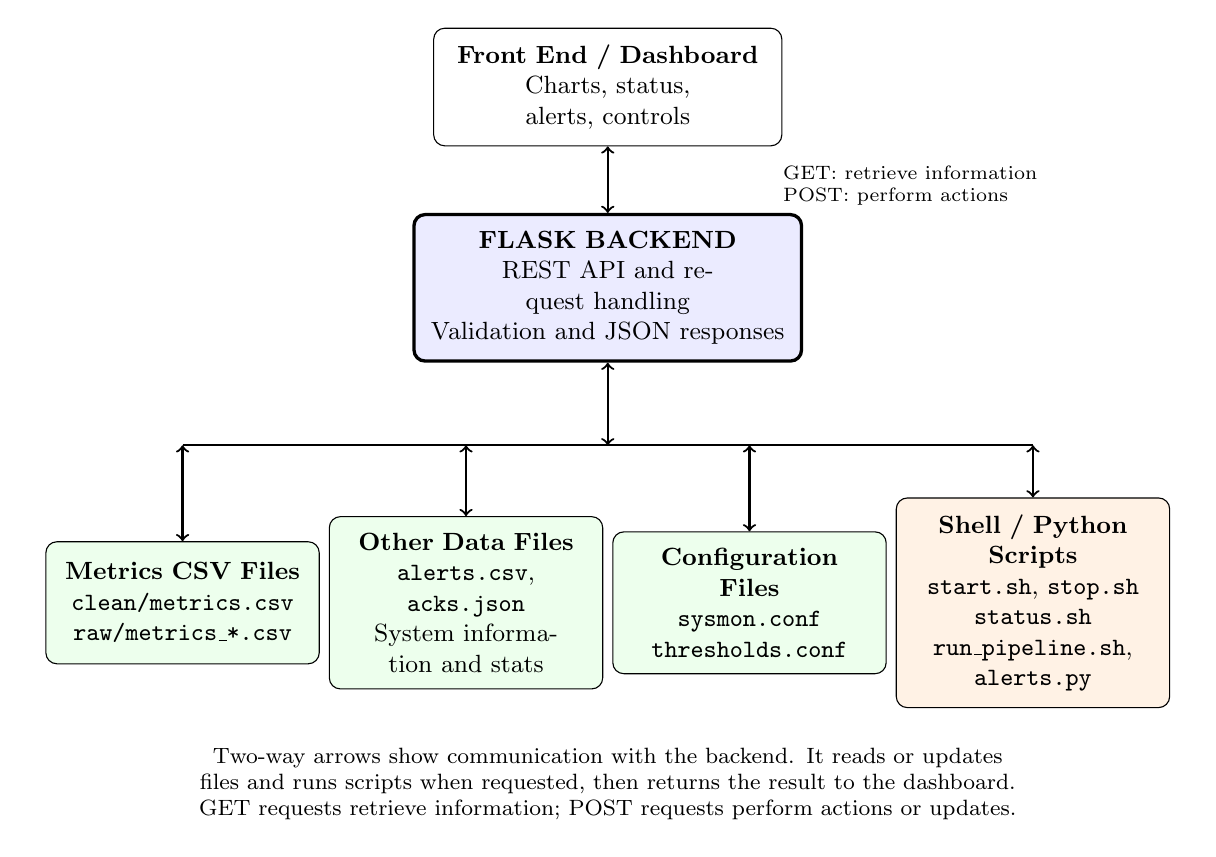
\begin{tikzpicture}[
  font=\small,
  box/.style={draw,rounded corners,align=center,inner sep=6pt,
              text width=3.05cm,minimum height=1.55cm},
  backend/.style={box,very thick,fill=blue!8,text width=4.5cm,
                  minimum height=1.25cm},
  frontend/.style={box,fill=white,text width=4.0cm,
                   minimum height=1.05cm},
  file/.style={box,fill=green!7},
  script/.style={box,fill=orange!10},
  link/.style={<->,thick},
  bus/.style={thick}
]

% Front end and central backend
\node[frontend] (ui) at (0,6.1)
  {\textbf{Front End / Dashboard}\\Charts, status, alerts, controls};
\node[backend] (api) at (0,3.55)
  {\textbf{FLASK BACKEND}\\REST API and request handling\\Validation and JSON responses};

% Files and scripts, spaced evenly below the backend
\node[file] (metrics) at (-5.4,-0.45)
  {\textbf{Metrics CSV Files}\\\texttt{clean/metrics.csv}\\\texttt{raw/metrics\_*.csv}};
\node[file] (other) at (-1.8,-0.45)
  {\textbf{Other Data Files}\\\texttt{alerts.csv}, \texttt{acks.json}\\System information and stats};
\node[file] (config) at (1.8,-0.45)
  {\textbf{Configuration Files}\\\texttt{sysmon.conf}\\\texttt{thresholds.conf}};
\node[script] (scripts) at (5.4,-0.45)
  {\textbf{Shell / Python Scripts}\\\texttt{start.sh}, \texttt{stop.sh}\\\texttt{status.sh}\\\texttt{run\_pipeline.sh}, \texttt{alerts.py}};

% Front-end requests
\draw[link] (ui.south) -- (api.north);
\node[font=\scriptsize,align=left,fill=white,inner sep=2pt,anchor=west]
  at (2.15,4.85) {GET: retrieve information\\POST: perform actions};

% Shared connection bus from backend to the four resource groups
\draw[link] (api.south) -- (0,1.55);
\draw[bus] (-5.4,1.55) -- (5.4,1.55);
\draw[link] (-5.4,1.55) -- (metrics.north);
\draw[link] (-1.8,1.55) -- (other.north);
\draw[link] (1.8,1.55) -- (config.north);
\draw[link] (5.4,1.55) -- (scripts.north);

% Explanation below the diagram
\node[align=center,text width=14.5cm,font=\footnotesize]
  at (0,-2.75)
  {Two-way arrows show communication with the backend. It reads or updates
   files and runs scripts when requested, then returns the result to the
   dashboard. GET requests retrieve information; POST requests perform
   actions or updates.};
\end{tikzpicture}
\end{center}

\textit{In summary: the dashboard does not directly manage the data files or run the system scripts. It sends a request to the backend; the backend acts as the controlled coordinator, works with the files or scripts, and returns the result.}
